
In this section, we introduce the details about Phoenix\footnote{https://github.com/dusk-network/phoenix-core}, the transaction model used by Dusk Network. 

\subsection{Overview of Phoenix}

Dusk Network is an open-source public blockchain with a UTXO-based architecture that allows the execution of obfuscated transactions and confidential smart contracts. In Phoenix, UTXOs are called {\textit{notes}}, and the network keeps track of all these notes by storing their hashes in the leaves of a \textit{Merkle tree of notes}. In other words, when a transaction is validated, the network includes the hashes of the new notes to the leaves of this tree. 

All transactions include a ZKP called \textsf{tx\_proof} that proves that the transaction has been performed following the network rules. Essentially, what this ZKP does is the following: first, it nullifies a note that the user is willing to spend. Second, proves that the user knows the value of a new note to mint, that will be sent to the receiver. Finally, proves that the amount of Dusk coins nullified is equal to the amount of coins created.

Greater details about the parameters included in the transaction have been skipped here, for the sake of completeness. Nevertheless, the next subsections explain how the protocol manages the notes nullification and minting, by introducing first the different keys the users have to handle.

\subsection{Protocol Keys}
\label{sec:protocol-keys}

In Phoenix, we have different kinds of keys. First, we have the static keys that belong to each user of the network, and we introduce them here as follows. Let $G, G'\gets\mathbb{J}$ be two JubJub points acting as our generators. We denote by $\hp$ and $\hb$ the Poseidon and BLAKE2b hash functions, respectively. Each user computes the following keys:

\begin{itemize}
	\item \textbf{Secret key:} $\sk = (a,b)$, where $a,b\gets \F_t$.
	\item \textbf{Public key:} $\pk = (A,B)$, where $A = a G$ and $B = b G$.
\end{itemize}

As noticed, Phoenix uses two-element keys, which allows users of the network to delegate the process of scanning for the notes addressed to them.

On the other hand, each note is associated with a unique one-time key pair (an approach introduced in~\cite{van2013cryptonote}), instead of using the static public key of the receiver, which hinders traceability. 

The computation of these keys is based on the Diffie--Hellman key exchange protocol \cite{diffie1976new}. The note public key of a note sent to a receiver with public key pair $\pk = (A,B)$, and its associated note secret key, are computed as follows:

\begin{itemize}
	\item \textbf{Note public key:} a sender willing to send money to a receiver whose public key $\pk = (A,B)$ is known by them in advance, must first compute a note public key $\npk$ following next steps.

	\begin{enumerate}
		\item Sample $r$ uniformly at random from $\F_t$.
		\item Compute a symmetric Diffie--Hellman key $\kdh = rA$.
		\item Compute a one-time public key $\npk = \hb(\kdh)G + B$.
		\item Compute $R = rG$.
	\end{enumerate}
	
	The sender of a note will attach to it the note public key $\npk$ and the partial Diffie--Hellman $R$ used to create $\npk$. Given a pair $(\npk, R$), the receiver can identify whether the note was sent to them by recomputing $\tkdh = aR$ (using their secret $a$), and checking the equation 

	\[\npk \stackrel{?}{=} \hb(\tkdh) G + B.\]
	
	\item \textbf{Note secret key:} the receiver can compute the note secret key $\nsk = \hb(\kdh) + b$, to be used when willing to spend that note. This key can only be computed by the receiver of the note since they are the only ones holding the whole secret key $\sk=(a,b)$, and $\sk$ cannot be recovered from public information. This is due to the discrete logarithm assumption in $\mathbb{J}$.
\end{itemize}

\subsection{Protocol Details}
\label{sec:transaction-model}

A note is defined as the following set of elements:

$$\Note = \{\type, \com, \pos, \nonce, \enc, \npk, R\}.$$

where $\type$ indicates the type of the note, either transparent or obfuscated; $\com$ is a commitment to the value of the note; $\pos$ is the position of the note in the Merkle tree of notes; $\nonce$ is an initialization vector needed for the encryption scheme; $\enc$ is an encryption of the opening of $\com$ that can be decrypted using the receiver's view key; $\npk$ is the note's public key, whose associated private key $\nsk$ can only be computed by the receiver of the note; and $R$ is a point in the Jubjub subgroup $\mathbb{J}$ that allows the receiver to compute $\nsk$ and also identify that they are the receiver of the transaction.

We describe Phoenix in the general scenario in which a sender wishes to send different amounts of money $\vnew{1},\dots,\vnew{n}$ to different receivers with public keys $\mathsf{pk_1},\dots,\mathsf{pk_n}$. We assume the sender owns a set of notes $\{\nold{1},\dots,\nold{m}\}$ each with an associated amount $\vold{i}$ such that \[\sum_{i = 1}^m \vold{i} \geq \sum_{i = 1}^n \vnew{i},\] i.e. the sender has enough funds.

When creating the transaction to transfer the funds, the sender will have to nullify the set of old notes being spent and mint a new set of notes $\{\nnew{1},\dots,\nnew{n}\}$ with the corresponding values $\vnew{i}$, and assigned to the corresponding receivers. 
The most common case is $\mathsf{n} = 2$, where a sender generates a note $\nnew{1}$ with value $\vnew{}$ for a receiver, and a second note $\nnew{2}$ for themselves with value  
$\change = \vnew{} - \sum_{i=1}^m\vold{i}$. 

To mint a new note for a receiver whose static public key is $\pk$, we first compute the note public key $(\npk, R)$ of the receiver as described in Section~\ref{sec:protocol-keys}. Next, we need to set the type of the transaction: if the transaction is transparent, we set $\type = 0$, and if the transaction is obfuscated, we set $\type = 1$. We also set $\vnew{}$ to the amount of money of the new note $\Note{}$. Finally, we need to commit to $\vnew{}$, and encrypt the opening as well. To do so, we first set a blinding factor for the commitment and a nonce for the encryption:

\begin{itemize}
	\item If $\type = 0$, set $s = 0$ and $\nonce = 0$.
	\item If $\type = 1$, set $s \leftarrow \F_{t}$ and $\nonce \leftarrow \F_t$.
\end{itemize}

and compute the value commitment $\com = \mathsf{Com}_\ck(v;s)$. Then, we encrypt the opening of $\com$:

\begin{itemize}
	\item If $\type = 0$, then set $\enc = \vnew{}$.
	\item If $\type = 1$, then 
	$\enc = \Enc_{\kdh} (\vnew{}||s; \nonce)$.
\end{itemize}

Now, we can set the new note to \[\Note = \{\type, \com, \nonce, \enc, \npk, R\}.\]

The next step is to compute a ZKP using the circuit depicted in Figure~\ref{fig:circuit} to prove the following elements:

\begin{itemize}
	\item \textbf{Membership}: the sender must prove that every $\mathsf{N}\in\{\nold{i}\}_{\mathsf{i} = 1}^{\mathsf{m}}$ is included in the Merkle tree of notes. To do so, the sender provides a Merkle proof for $\hp(\mathsf{N})$, and the circuit verifies the Merkle proof in \texttt{verify\_merkle\_proof()}. We observe that all these inputs are private and hence, the proof will not reveal which note is being spent, only that it belongs to the Merkle tree of notes. 

	\item \textbf{Ownership}: the sender must prove that they hold the note secret key $\nsk$ of every note $\mathsf{N}\in\{\nold{i}\}_{\mathsf{i} = 1}^{\mathsf{m}}$. 
	Instead of including their private key as an input to the circuit and computing $\npk$ inside, the sender proves (using the \texttt{verify\_signature()} box inside the circuit) that they can sign a message with that key. In this case, they use the double-key Schnorr signature scheme to sign the hash of the transaction. 

	\item \textbf{Nullification}: the sender must prove that $\nullifier=\hp(\npk' || \pos)$. Note that the sender provides the nullification key $\npk' = \nsk G'$ as an input to the circuit and not the note secret key $\nsk$. As we just explained, the double-key Schnorr signature guarantees that $\npk'$ is indeed $\nsk G'$. The result of the \texttt{hash()} box is the nullifier, which is a public output of the circuit that is later included as part of the transaction.
	
	\item \textbf{Balance integrity}: the \texttt{verify\_balance()} box checks that 
	\begin{equation}\label{eq:balance}
		\sum_{i = 1}^m \vold{i} - \sum_{i = 1}^n \vnew{i} - \mathsf{gas} = 0,
	\end{equation} where $\mathsf{gas}$ is the maximum amount of gas that the sender is willing to pay for the transaction.
\end{itemize}

\begin{figure}[h]
	\centering
	\setlength{\fboxsep}{5pt}%
	\setlength{\fboxrule}{0.3pt}%
	\fbox{
		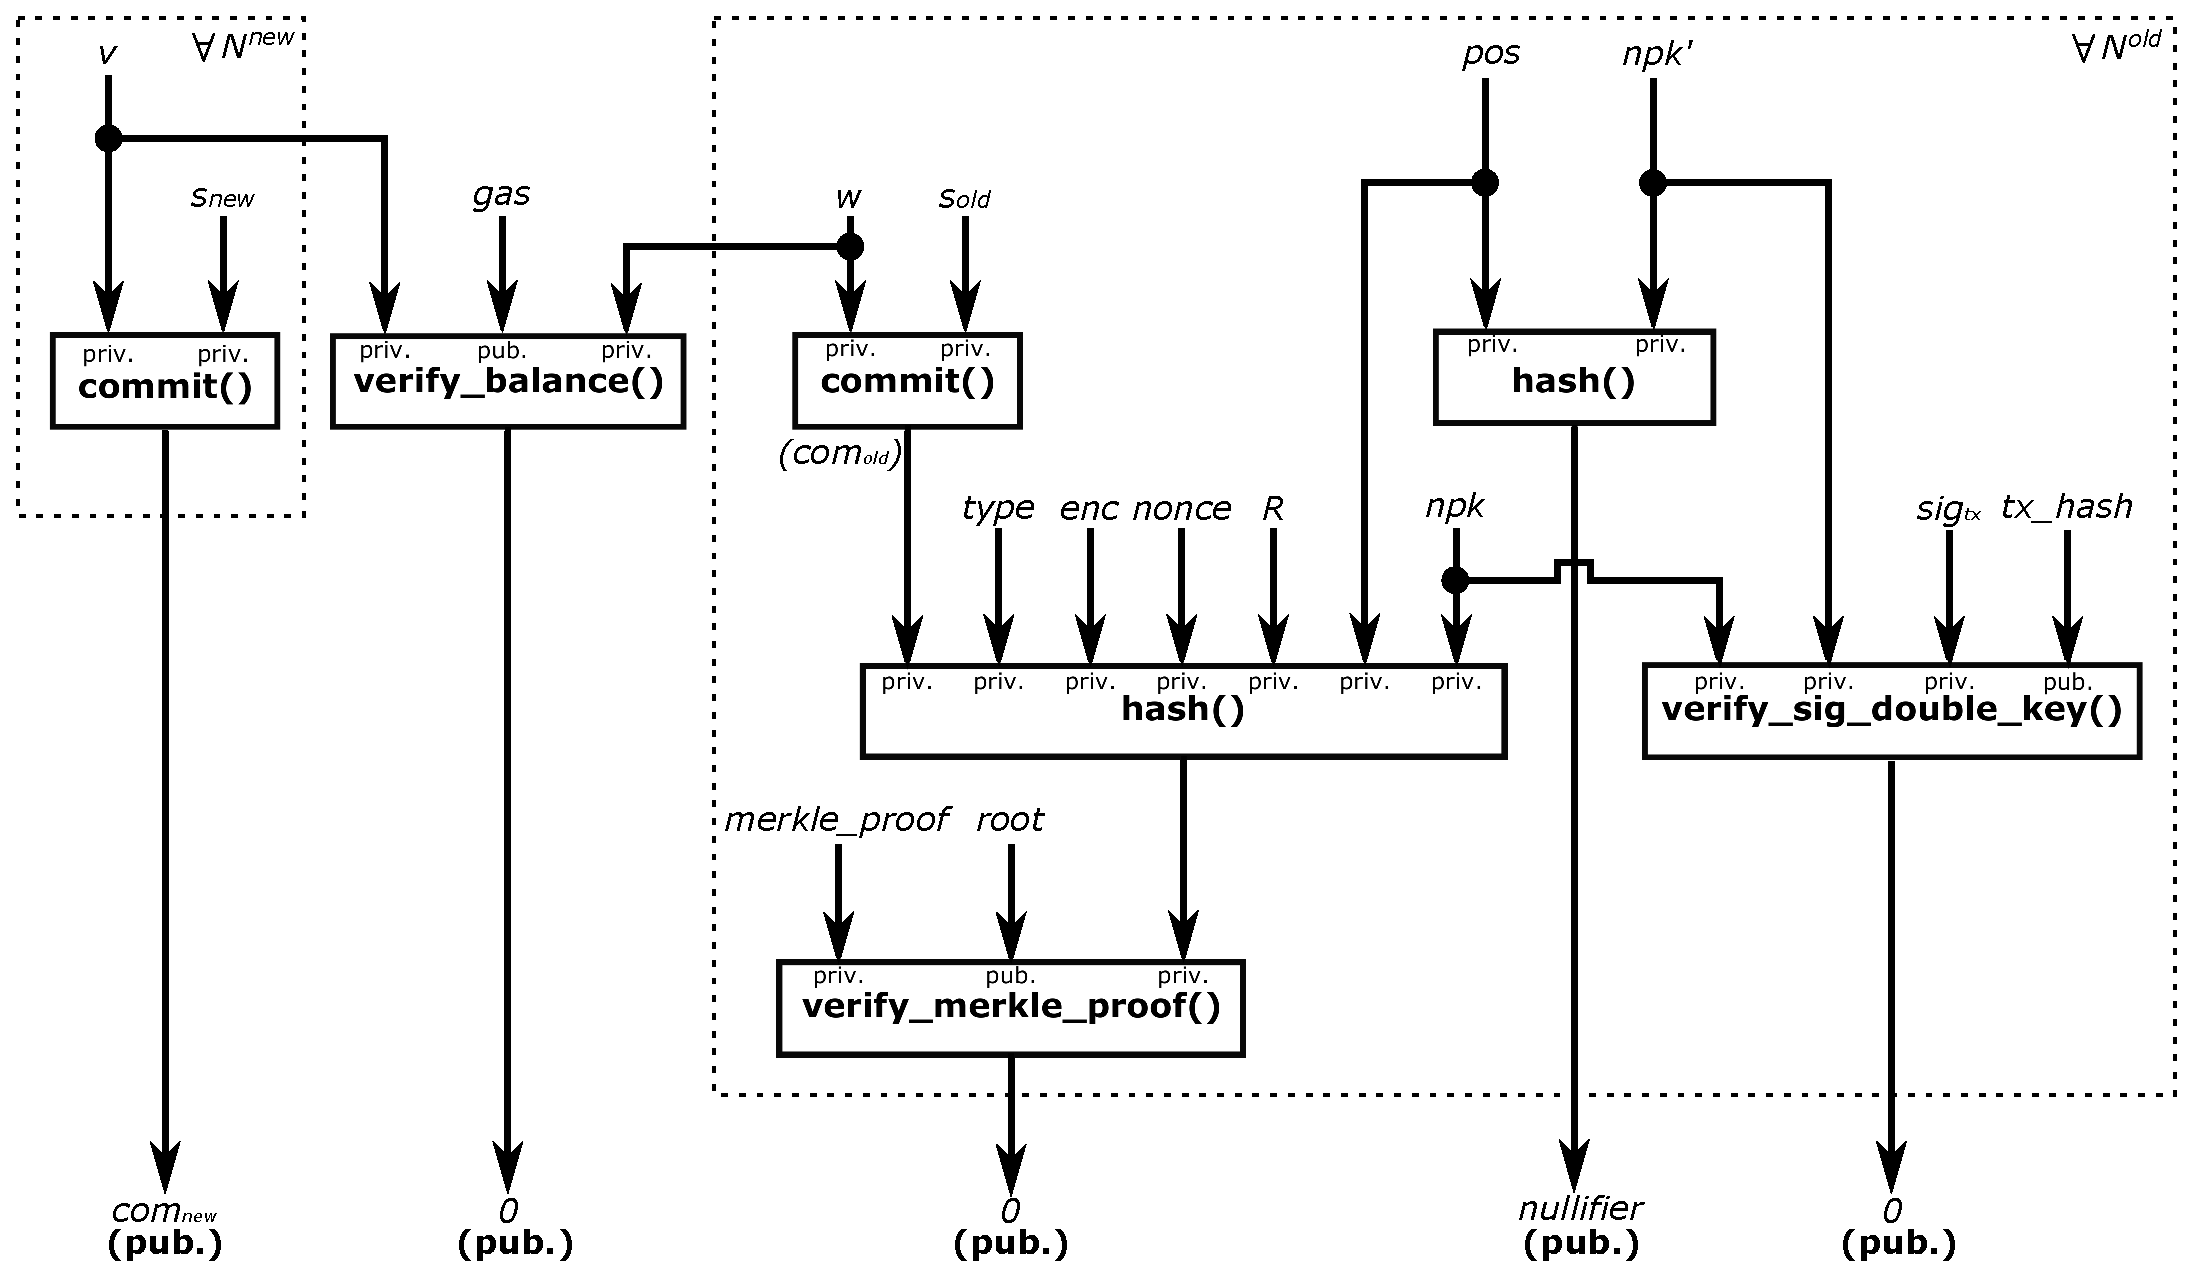
\includegraphics[width=460pt,draft=false]{images/circuit_plus.eps}}
	\caption{Arithmetic circuit for a Dusk transaction proof.}
	\label{fig:circuit}
\end{figure}

Observe that using the double-key Schnorr signature as proof that the user holds $\nsk$, allows users to delegate the generation of the ZKP to a partially trusted third party, that is, a \textit{proof helper}. This delegation would require the user to entrust the old and new values of the notes to the proof helper, but not their secret key. 

Finally, the remaining checks not verified inside the circuit are performed by the network. For instance, checking that the nullifier included in the transaction matches the output of the circuit, or that the note has the right typeset.




